%
% File acl2016.tex
%
%% Based on the style files for ACL-2015, with some improvements
%%  taken from the NAACL-2016 style
%% Based on the style files for ACL-2014, which were, in turn,
%% Based on the style files for ACL-2013, which were, in turn,
%% Based on the style files for ACL-2012, which were, in turn,
%% based on the style files for ACL-2011, which were, in turn, 
%% based on the style files for ACL-2010, which were, in turn, 
%% based on the style files for ACL-IJCNLP-2009, which were, in turn,
%% based on the style files for EACL-2009 and IJCNLP-2008...

%% Based on the style files for EACL 2006 by 
%%e.agirre@ehu.es or Sergi.Balari@uab.es
%% and that of ACL 08 by Joakim Nivre and Noah Smith

\documentclass[11pt]{article}
\usepackage{acl2016}
\usepackage{times}
\usepackage{url}
\usepackage{latexsym}
\usepackage{xcolor}
\usepackage{latexsym}
\usepackage{tabularx} 
\usepackage[english]{babel}
\usepackage{multirow}
\usepackage{booktabs}
\usepackage{ifthen}
\usepackage{tikz,pgfplots}
\usepackage{xcolor,colortbl}
\usepackage[color=cyan]{todonotes}

\newcommand{\DEVELOPMENT}{1} % 1= show comments, 0=no comments
\usepackage{ifthen}
\ifthenelse{\DEVELOPMENT = 1}{
	\newcommand{\tz}[1]{\textcolor{cyan}{\textbf{TZ:} #1}}		
	\newcommand{\mw}[1]{\textcolor{red}{\textbf{MW:} #1}}				
}{
	\newcommand{\tz}[1]{}		
	\newcommand{\mw}[1]{}			
}


%\aclfinalcopy % Uncomment this line for the final submission
%\def\aclpaperid{***} %  Enter the acl Paper ID here

\setlength\titlebox{4cm}
% You can expand the titlebox if you need extra space
% to show all the authors. Please do not make the titlebox
% smaller than 5cm (the original size); we will check this
% in the camera-ready version and ask you to change it back.

\newcommand\BibTeX{B{\sc ib}\TeX}

\title{Mining Implicit Argumentation in Social Media --  \\ Status Quo}

\author{Michael Wojatzki}

\date{}

\begin{document}
\maketitle
\begin{abstract}
This status quo document has the following structure:
First, we will give a brief overview on the field of Argument Mining, outline problems we identified and state our research questions.
Second, we describe our model, which is robust against these problems.
Afterwards, we will show results of experiments which were conducted to examine the quality and usefulness of our model.
Finally, we will address remaining questions and problems we see in our approach and the so far conducted experiments. 
\end{abstract}



\section{Overview on State-of-the-Art and RQs}

Argumentation is a constellation of propositions that is used to convince someone of a standpoint.
Especially in social media, argumentation is frequently observable and can be considered as an essential element of social media interaction such as online debates.
Since this phenomenon occurs at a massive scale, many groups of information seekers (e.g. researchers, journalists, companies, etc.) could benefit from an automated analysis of social media argumentation.
This automated identification of argumentative structures within written communication is called argument mining \cite{green2014argmining}.

Typically, models of argument mining assume that an argument consists of at least an explicit \textit{claim} and a number of optional supporting structures such as \textit{premises} \cite{palau2009argumentation,peldszus2013ranking}.
Depending on which theory of argumentation (e.g. \newcite{toulmin2003uses} or \newcite{freeman1991dialectics}) the approaches follow, this structures are more or less specialized.

%\begin{figure*}[hbt]
%\centering
%  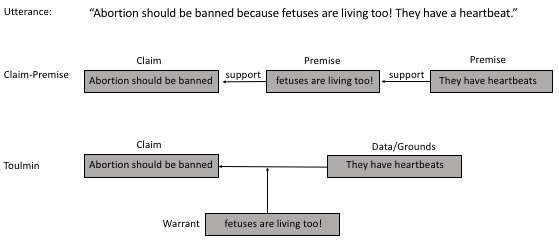
\includegraphics[width=.8\textwidth]{figures/claim_premise_toulmin.png}
%  \caption{Schemes for modelling arguments according to \newcite{toulmin2003uses} and the common \textit{claim}-\textit{premise} scheme.}
%\end{figure*}

After analysing the state-of-the-art, we identified two fundamental problems of current approaches.
First, text harvested from social media is usually shorter, less dense for arguments, noisy and the used arguments are often not as sophisticated.
Second, in contrast to elaborated text, social media contains a high proportion of implicit argumentation (e.g. as annotated in the corpora by \newcite{habernal2014argumentation} or \newcite{boltuzic2014back}) and is done on the basis of shared assumptions.


For instance, in a debate on atheism, one may observe an utterance such as \textit{Bible: infidels are going to hell} or even shorter \textit{\#JesusOrHell}.
In the context of a debate about atheism, both utterances implicitly express the argument that the author is against atheism, because the bible says that this will result in a stay in hell after death.
However, both claims are never explicitly mentioned.

In order to tackle the described problems, we propose stance-based argument mining as an alternative scheme for modelling arguments.
A stance is the attitude (being in favor or against) of an author towards a given target like a politician or a controversial topic \cite{StanceSemEval2016}.
By transforming propositions into a constellation of stances towards targets, one should obtain a more abstract representation of arguments that should be more robust against implicitness and noise.

\begin{figure}
%\centering
   %\frame{
  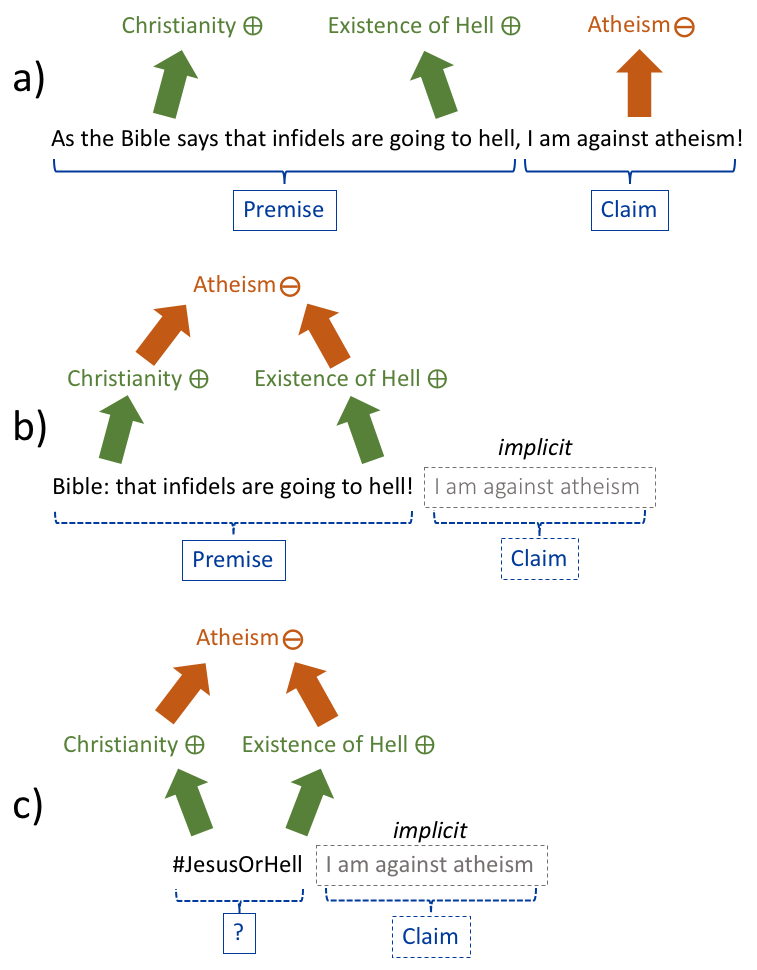
\includegraphics[width=0.49\textwidth]{figures/comparison_models_2.png}
  %}
  \caption{Stance-based vs.\ \textit{claim}-\textit{premise} model}
  \label{fig:comparison_models}
\end{figure}

\section{Stance-Based Argument Mining}
\label{sec:our_model}

In order to solve the major challenge of implicit arguments that cannot be modelled well with existing approaches, we introduce a new model based on a \textit{debate stance} that will in most cases be implicit, but can be inferred from one or more \textit{explicit stances} that rely on textual evidence from the utterance.
We thereby assume that an utterance is always made in the context of a certain debate.

Figure~\ref{fig:icebergModel} gives on overview of the model which we metaphorically describe as an iceberg.

\begin{figure}
%\centering
   %\frame{
  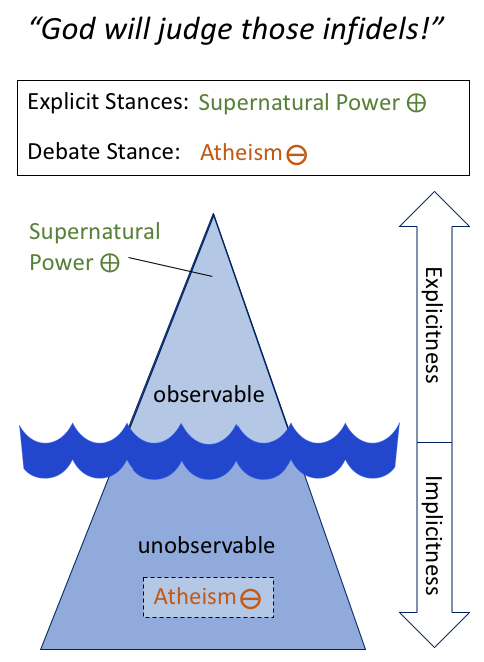
\includegraphics[width=0.49\textwidth]{figures/IceBergModel_single.png}
  %}
  \caption{Our model and the iceberg metaphor for capturing implicit argumentation by using the the components (i) explicit stances and (ii) a debate stance.}
  \label{fig:icebergModel}
\end{figure}

In the context of a debate about atheism, an utterance like \textit{God will judge those infidels!} is like the visible (explicit) part of the iceberg.
It expresses a stance in favor of a supernatural power (\textit{Supernatural Power}\,$\oplus$), while the actual stance on the debate target of atheism (\textit{Atheism}\,$\ominus$) is not visible but must be inferred.
Note that the debate stance might also be explicitly expressed (see figure~\ref{fig:comparison_models}a), but in implicit argumentation it has to be derived from the explicit stances.

In principle, each utterance evokes a large set of implicit stances (in a similar way as the iceberg contains a lot of invisible ice below the waterline). 
For instance, one may infer that a person uttering \textit{Bible: infidels are going to hell!} is probably in favor of praying and might have a negative stance towards issues such as abortion, same-sex marriage, etc. 
However, we argue that being in favor of Christianity already implicitly covers these stances under a common sense interpretation. 
Depending on the present informational need these targets may be more or less relevant.

An explicit stance always implicitly covers a large variety of associated stances, we propose the metaphor of an iceberg, whose actual size is also not observable but present and significant under the water surface. 

A stance which may be expressed only implicitly and may be inferred from the explicitly made stances is the second component of our model -- namely the debate stance.
This stance is important for the expressiveness of of our model, since it corresponds to the claim of other models in argument mining.

Note, that the debate stance and other stances that are implicitly covered by the explicit stances are derived as a function of the context of the present debate. 
They may be a completely different if one states the same utterance in a different debate.
The two layers of the model and the iceberg metaphor are exemplified in figure~\ref{fig:icebergModel} for an utterance with one explicit stances. 

\paragraph{Debate Stance}
As described above, we refer to the (frequently implicit) stance towards the target of the whole debate as \textit{debate stance}.
For instance, if in the context of an atheism debate someone describes their personal faith, we may assume that they want to communicate the fact that they are against atheism.
Note that exactly the same utterance might not communicate a stance against atheism in the context of another debate such as on the importance of charity.

\paragraph{Explicit Stances}
While the overall debate stance may be implicit, there has to be some explicit information in the utterance that enables this inference.
Otherwise the goal of the persuasive utterance (i.e.\ convincing someone or at least expressing her standpoint) cannot be achieved.
As a stance can always be transformed into a claim which can be considered as the minimum constituent of an argument \cite{habernal2014argumentation,palau2009argumentation}, we argue that the minimal information that has to be provided in a persuasive utterance is a stance towards some target.

Given a stance, humans can infer the argument using a common sense interpretation.
If one states \textit{God will judge those infidels} (\textit{Believe in God}\,$\oplus$) in an atheism debate, one can infer stances such as \textit{being a infidel is a sin}\,$\oplus$, \textit{God punishes infidels}\,$\oplus$ and the debate stance \textit{Atheism}\,$\ominus$.
If an author wants to deviate from this interpretation, they need to communicate this explicitly, e.g.\ by adding \textit{but the constitution grants religious freedom} (\textit{religious freedom}\,$\oplus$). 

%From lexical priming studies it is known that the perception of words can activate knowledge about associated concepts or real-world events \cite{jones2012lexical,hare2009activating}.
%Since there is also strong evidence for priming effects of stimuli other than words \cite{tulving1990priming}, we conclude that priming should be applicable to stances as well and therefore forms the underlying mechanism of implicit argumentation.

The granularity of the stance targets has thereby to be considered with respect to the present informational needs.
If one wants to get a more general view on the examples in figure~\ref{fig:comparison_models}, one could fall back to the target \textit{belief in a supernatural power} which is also less explicitly covered.
%Analogously, the unobservable parts of the argument vary in the degree of their implicitness.
%The degree of implicitness is seen here as the strength to which other stances are primed by the explicit part.
%For instance, if one claims the existence of hell, one affirms the existence of heaven with a small degree of implicitness but a stance about reincarnation is taken only very implicitly.
As demonstrated by \newcite{conrad2012recognizing}, a too fine grained distinction has the consequence of a sparse distribution which makes it difficult to derive relations between components of their model or to enable automated classification.
Thus, selecting the most explicit targets does not appear to be the appropriate level to gain comprehensive insights on how taking a stance in a debate is manifested by explicit stances.
However, if a target is too implicit, it might be invoked by authors in favor of the debate target as well as against the target.


\section{Conducted Experiments and Results}
Now we report on previously conducted experiments that shed light on certain aspects of the model.
First, we examined how well stance can be recognized in general.
Second, we have made a first attempt to instantiate a stance-based model for argument mining.

\subsection{Automated Stance Detection}
\label{sec:semeval}
Being able to automatically detect and classify stance in social media is important for a deeper understanding of debates and would thus be a great tool for information seekers such as researchers, journalists, customers, users, companies, or governments.
In addition, such analysis could help to create summaries, develop a deeper understanding of online debating behavior, identify social or political groups, or even adjust recommendations to users' standpoints \cite{anand2011cats,sridhar2014collective,boltuzic2014back}.
In addition, for the development and feasibility of a argument mining scheme which is based on stance the ability to detect and classify stance is crucial.

Therefore, we participated in the \textit{\mbox{SemEval} 2016 Task 6: Detecting Stance in Tweets} which represents the first shared task on stance detection that tries to explore the current state-of-the-art.
The task defines stance relative to a given target like a politician or a controversial topic.
A text can then either be in favor of the given target ($\oplus$), or against it ($\ominus$).
As the dataset also contains texts without a stance, we additionally have to deal with the the class \textsc{none}.

Figure \ref{fig:sketch1} gives a overview on our system for automated stance detection (for a a more detailed explanation see \newcite{wojatzki2016stance}).

\begin{figure*}
  \centering
  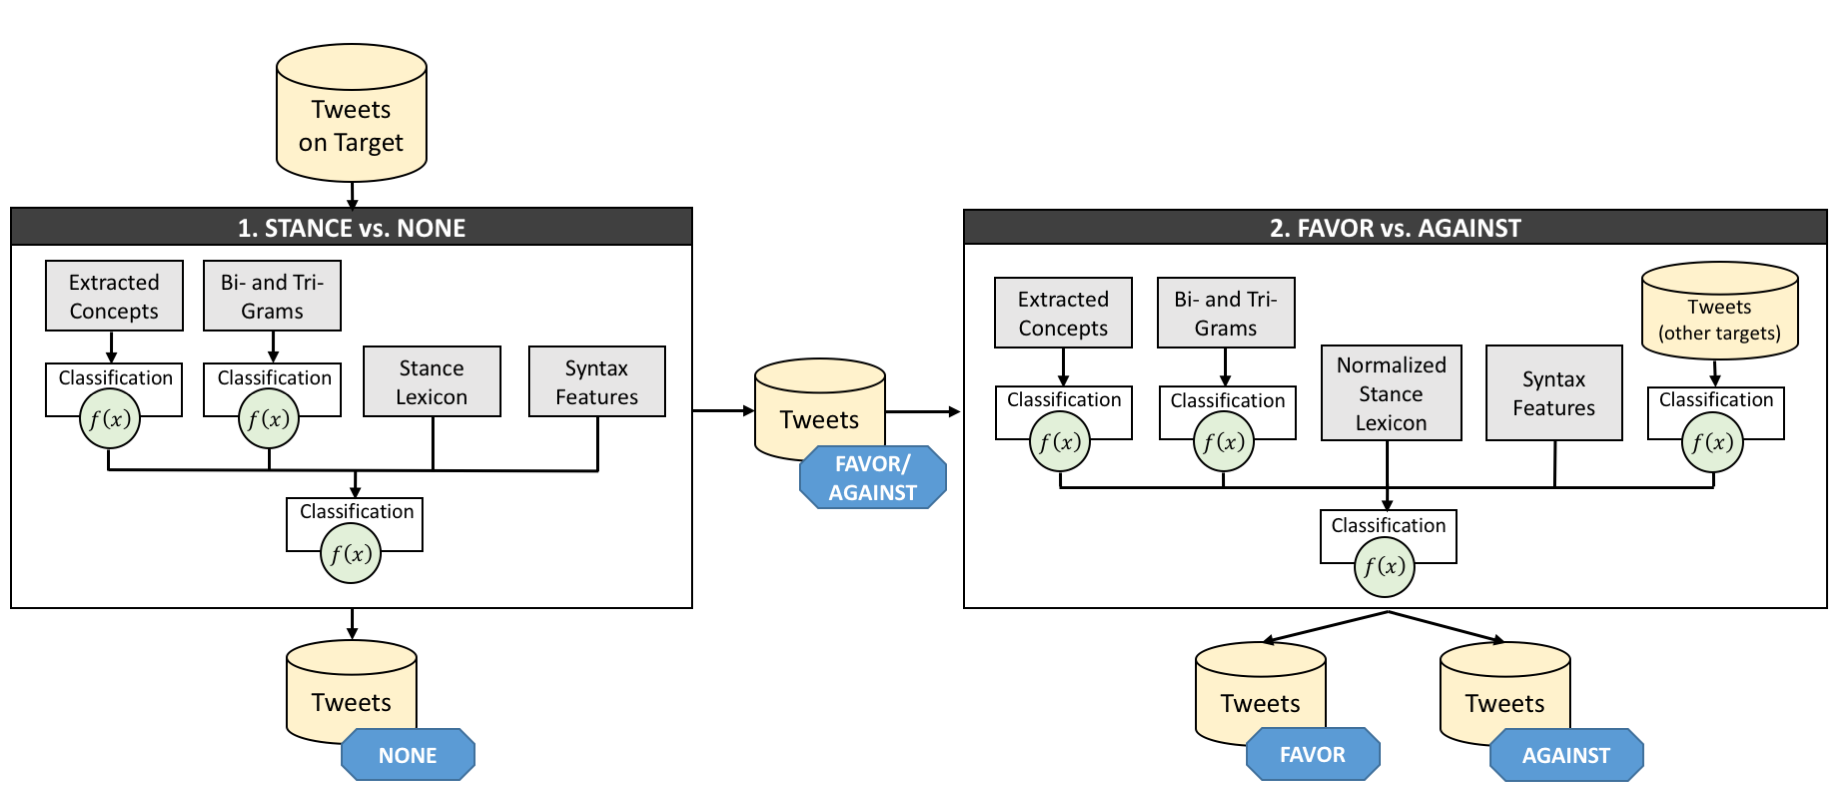
\includegraphics[scale=0.25]{figures/stance_skizze_new.png}
  \caption{Overview on the sequence of stacked classifications that is used for the supervised setting (subtask A)}
  \label{fig:sketch1}
\end{figure*}

The goal of this task is to classify tweets about five targets: \textit{Atheism}, \textit{Climate Change is a Real Concern}, \textit{Feminist Movement}, \textit{Hillary Clinton}, and \textit{Legalization of Abortion}.
For each target, there are about 400-600 manually labeled tweets that can be used for training.

As the targets are quite different, we train a separate classifier for each of them. 
Additionally, we split the three-way classification into a stacked classification, in which we first classify whether the tweet contains any stance (classes $\oplus$ and $\ominus$) or no stance at all (class \textsc{None}).
In a second step, we classify the tweets labeled as containing a stance as $\oplus$ or $\ominus$.
Our analysis revealed that simple word features are best suited to learn the relationship between tweets and stance.

Other teams in the task used comparable feature sets, but relied on different machine learning techniques that may be summarized as deep learning. 
However, as demonstrated by the task organizers none of them beats the provided baseline which is  a support vector machine equipped with character and word ngrams \cite{StanceSemEval2016}.
In a post-hoc analysis they show that this baseline profits from leveraging unlabelled data \cite{mohammad2016stance}.
In general, the results suggest that the performance of the state-of-the-art is significantly better than a random or a majority class baseline, but still leaves huge room for improvements.


\subsection{Explicit and Implicit Stances}
After we have dealt with the debate stance alone, we have made a first attempt to instantiate a model for stance based argument mining.
Therefore, we conducted a study with three annotators in which we annotetd tweets with a debate stance and stances towards explicit targets (for more detail see \newcite{wojatzki2016stanceBased})

As described in section \ref{sec:our_model}, one has to consider the tradeoff between the sparsity of explicit targets and their expressivness.
For this first attempt, we utilize a semi-automated, bottom-up approach for finding a list of explicit targets.
Consequently, we examine the frequency distributions of nouns and named entities.
Since we observe that the distribution follows Zipf's law, we expect that words with a frequency above the long tail, can serve as candidates as they occur frequently enough to avoid the sparsity problem.

As we want to ensure that the targets used enable us to differentiate the authors' positions sufficiently, we also consider the degree of association between nouns and named entities to the stances \textit{Atheism}\,$\oplus$ and \textit{Atheism}\,$\ominus$.
In detail, we compute the collocation coefficient $Dice$ \cite{smadja1996translating} for each word, and selected the 25 words which are most strongly associated with \textit{Atheism}\,$\ominus$ and \textit{Atheism}\,$\oplus$.

We found the resulting concepts to be too numerous and too fine-grained to be used in our model.
We thus, manually group concepts into more coarse-grained targets.
For instance, concepts such as \textit{Bible} and \textit{Jesus} are grouped into the target \textit{Christianity}.
A potential criticism of our approach is that at this stage of our work, we can not evaluate whether the set is best possible choice.

\subsubsection{Annotation}
Again we rely on data used by the described SemEval task which enables us to consider the present work in this context.
A relevant property of the data, as stated by the task organizers, is that it contains a high proportion of tweets that do not explicitly mention the target and therefore can be considered as implicit utterances.
We limit our study to 733 tweets on \textit{Atheism}, as we found the topic to require less knowledge about specific political events.

In order to familiarize the annotators with our scheme, we previously trained them on a small data set that is comparable in its social media character but concerns a different target.  
Since it is possible that our annotators interpret the tweets differently than in the original annotation, we re-annotated the (overall) debate stance using the original questionnaire described in \newcite{StanceSemEval2016}.
While annotating explicit stances, the annotators had the instruction to only annotate stances towards targets if they have textual evidence for it.

\subsubsection{Inter Annotator Agreement}

\begin{figure*}[ht!]
\centering
\begin{tikzpicture}
        \begin{axis}[
        xbar,
            symbolic y coords={No Evidence,  Life After Death, Same-Sex Marriage, Religious Freedom, USA, Conservatism, Freethinking,no explicit target, Supernatural Power, Secularism, Islam, Christianity, , Atheism},
            ytick=data, 
            bar width= 5,
            width=.8\textwidth,
           % yticklabel style={rotate=45, anchor=east, align=center},
            height=.4\textwidth,
            xmin = 0, 
			xmax = 1,
			nodes near coords,
			enlarge y limits=0.04,
			xlabel=Fleiss' $\kappa$,
			yticklabel=\ifthenelse{\equal{\tick}{no explicit target}}{\textit{no explicit target}}{\tick}]
          ]
            \addplot[xbar,fill=blue] coordinates {
            	(0.72,Atheism)
                (0.85,Christianity)
                (0.81,Islam)
                (0.76,Secularism)
				(0.73,Supernatural Power)
                (0.73,Freethinking)
                (0.73,no explicit target)
				(0.63,Conservatism)
                (0.57,USA)
                (0.52,Religious Freedom)
				(0.51,Same-Sex Marriage)
				(0.43,Life After Death)
				(0.31,No Evidence)
            };
        \end{axis}
       % \draw [ultra thick, dashed, draw=gray](2.2,4.8)--(2.2,0); %separator (is not positioned very clever at the moment)
    \end{tikzpicture}
    \caption{Inter-annotator agreement of the debate stance \textit{Atheism} and explicit stances}
\label{fig:kappa_subTargets}
   \end{figure*}
The notation of explicit targets should result in a strong agreement of the annotation of the debate stance because it enforces a deep analysis of the communicative goal of an utterance.   
As shown in figure~\ref{fig:kappa_subTargets}, we obtain a Fleiss' $\kappa$ of 0.72 for the annotation of the debate stance.

Two explicit targets (\textit{Christianity} and \textit{Islam}) yield especially high agreement, because they are associated with clear signal words such as \textit{Jesus} and \textit{Quran}.
Other targets such as \textit{Secularism} are rather abstract.
They hardly involve special signal words but still gain high agreements, which shows that our annotators did not just recognize certain keywords, but also reliably annotate more abstract targets.
An error analysis for the target \textit{Same-Sex Marriage} shows that there is disagreement if the tweet contains a stance towards gay rights in general but not to gay marriage.
We therefrom see two possibilities here to improve the agreement:
On the one hand, we could choose more comprehensive targets such as \textit{gay rights} to cover the combined positions.
On the other hand, we could train the annotators to more consistently account for such differences.
For other targets(e.g.\ \textit{No Evidence}), we observe that annotators sometimes deviated from our guidelines and incorporated different degrees of inferred knowledge as they used \textit{Bill Nye} or \textit{Richard Dawkins} as anchors for their decisions.

Finally, we obtain a $\kappa$ of 0.63 for the joint decision on both the debate and the explicit targets.

The obtained inter-annotator agreement shows that our model can be annotated reliably and that the recognized difficulties may be compensated by a better training of the annotators and a better selection of targets.
   
\subsubsection{Stance Pattern Analysis}

\begin{figure}[ht!]
\centering
  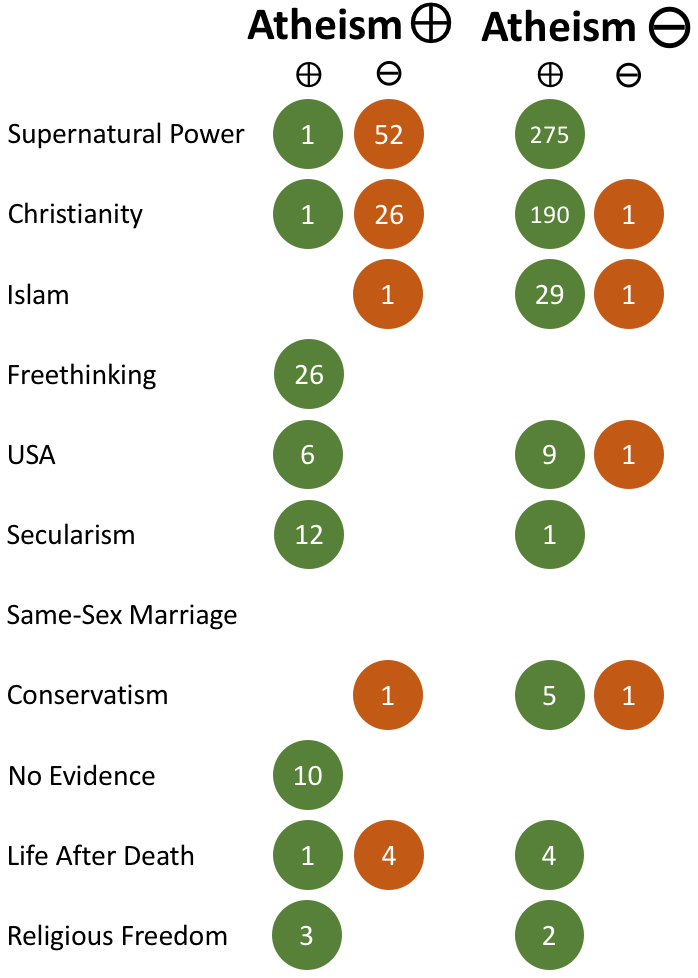
\includegraphics[width=0.45\textwidth]{figures/patterns_flat.png}
  \caption{Frequency of explicit stances grouped according to debate stance}
  \label{fig:patterns_flat}
\end{figure}

In order to inspect usage patterns of explicit stance taking, we must agree on one annotation for each tweet.
Since we do not assume that there are differences in the quality of the three annotators, we rely on a majority vote to compile a final annotation. 

Figure~\ref{fig:patterns_flat} visualizes the frequency of the explicitly taken stances for Atheism\,$\oplus$ and Atheism\,$\ominus$.
It shows that there are significant differences in the argumentation patterns between the two camps.
As expected, if advocates of atheism are against a target such as \textit{Christianity}, the opponents are mostly in favor of it or do not mention it.

From these analysis we can conclude that stable patterns of argumentation using explicit stances other than the debate stance exist.
This is a strong indication for the validity of our assumption that the debate stance can be inferred from explicitly expressed stances.


\subsubsection{Automatically Assigning Stances}
In order to investigate how well our model can be assigned automatically, we conduct classification experiments and compare with suitable baselines.
Based on how well the components are classifiable, we can derive how well the model is assignable as a whole.

We re-implement a state-of-the-art classifier as described in section \ref{sec:semeval}, run experiments in the manner of a ten-fold cross-validation and report micro averaged $F_1$.

\paragraph{Explicit Stances}

\begin{table}
\small
\centering
\begin{tabular}{lcc}
\toprule
\textbf{Target (\# instances)} & \textbf{Baseline}   & \textbf{SVM}    \\
\midrule
Supernatural Power (335)     & .53 & .78\\
Christianity (223)           & .69 & .79\\
Islam (43)                   & .94 & .95 \\
%\textit{Secularism (21)}    & \textit{.965} & \textit{.972} \\
%\textit{Conservative Movement (12)}  & \textit{.983} & \textit{.986}\\
%\textit{Religious Freedom (7)}    & \textit{.988} & \textit{.990}\\
%\textit{USA (28)}                   & \textit{.961}  & \textit{.964}\\
%\textit{No Evidence (10)}         & \textit{.986} & \textit{.987}\\
%\textit{Life After Death (9)}     & \textit{.987} & \textit{.987} \\
%\textit{Same-Sex Marriage (15)}    & \textit{.979} & \textit{.978}\\
%\textit{Freethinking (31)}         & \textit{.986} & \textit{.957}\\
\bottomrule
\end{tabular}
\caption{Explicit stance classification (only showing targets occurring in at least 5\% of all instances)}
\label{table:classificationExplicitStances}
\end{table}

Table~\ref{table:classificationExplicitStances} shows the results of the state-of-the-art classifier and the majority class baseline for comparison.
The results indicate that the two most frequent targets can be classified with success, if one relates them to the majority class baseline.
We observe that each target has its own linguistic markers such as the use of Arabic terms if one is in favor of Islam. 
Therefore, we argue that these peculiarities can be targeted even better by specialized features.

The analysis in table~\ref{table:classificationExplicitStances} excludes targets that have a insufficient coverage (less than 5\% of all instances) to train a meaningful model.
A possibility to deal with this sparsity may be to incorporate unlabelled data such as demonstrated for traditional models by \newcite{habernal2015exploiting} or \newcite{mohammad2016stance}.

\paragraph{Debate Stance}

\begin{table}[]
\small
\centering
\begin{tabular}{lc}
\toprule
Feature Set    & F$_1$ \\
\midrule
baseline       & .49            \\[5pt]
n-gram          & .66             \\
ngram + explicit stance$_{predicted}$ & .67            \\
ngram + explicit stance$_{oracle}$ &  .88      \\
explicit stance$_{predicted}$ & .65  \\
explicit stance$_{oracle}$ & .88  \\
\bottomrule         
\end{tabular}
\caption{Debate stance classification}
\label{table:classificationDebateStances}
\end{table}

Table~\ref{table:classificationDebateStances} shows the results obtained for automatically assigning the debate stance.
Besides the majority class baseline ($F_1=.49$), we use the same setup as for the explicit stances to train an n-gram based classifier and obtain an $F_1$ of $.66$.
In order to evaluate the usefulness of explicit stances for inferring the debate stance, we use the predictions from the previous experiment as features.
This stacked classifier performs on par ($.65$) with the n-gram based classifier.
It seems that the quality of predicting explicit stances is not yet good enough to improve over the state-of-the-art without incorporating general n-gram features.
To estimate the potential of explicit stance features for classifying the debate stance, we add an oracle condition to our experiments in which we assume that the classification of explicit stances is done correctly.
This classifier using only the manually annotated explicit stances yields an $F_1$ score of $.88$ showing that large improvements over the state of the art are possible if explicit stances can be more reliably classified.
We believe that this is indeed possible as explicit stances are always grounded in the text itself, while the debate stance might only be indirectly inferred.


\section{Remaining Problems}
The previously conducted experiments are only a first step towards argument mining that is robust against less elaborated and implicit arguments.
At the present time we identify three major lines of future work.  

\subsection{Advanced Machine Learning Techniques and Feature Engineering}
So far, we applied standard machine learning techniques ($SVM$ equipped with word n-grams) to the classification tasks.
At the moment we modelled the task as a document classification (i.e. the targets are classified independently).
Since we assume that there are strong dependencies between the targets, future experiments should implement a sequence classification by using e.g. $SVM_{HMM}$ of conditional random fields. 

As indicated by \newcite{habernal2015exploiting} and \newcite{mohammad2016stance} leveraging huge amounts of unlabelled data is beneficial for stance classification.
The idea behind this is to address the data sparsity with approaches such as bootstrapping or distant supervision.
In addition, the sparsity problem could be tackled by utilizing lexical semantic resources such as Wikipedia and semantic relatedness of words.
Consequently, we want to run experiments that implement these methods.

Moreover our model should profit from features that are tailored to certain explicit targets.
For instance, features that capture references passages by using regular expressions or text similarity measures towards the Bible should be beneficial for classifying the target \textit{Christianity}.

While the debate stance of an utterance is -- of course -- dependent on the current debate, models for classifying stance towards explicit targets should be domain more domain indepedent. 
Although this is an assumption that has to be proved, it is hard to imagine a domain in whichI love Jesus the utterance \textit{I love Jesus} does not express a favorization of \textit{Christianity}.
Consequently, it should be possible to create a collection of models for classifying explicit stances that could be applied to a new debate in the manner of a building block system.


\subsection{Selection of Explicit Targets}
In our model, choosing the right number and granularity of targets is crucial.
On the one hand, they have to be expressive enough to capture differences in nuanced argumentation.
On the other hand, they should not be too fine grained as this would result in very sparse distributions that cannot be handled by automated methods.
In our previous work \cite{wojatzki2016stanceBased}, we used a simple frequency approach that focussses on nouns and named entities only.
However, at the moment it is unclear how well the resulting set is able to describe the actually used explicit targets. 
Consequently, we want to examine this problem from three perspectives:
\begin{itemize}
  \item Gold Standards and Evaluation: Especially critical is to develop appropriate methods that allow to assess the performance of selection approaches. Therefore we need to create gold standard data and choose meaningful measures. We are currently looking for ideas to operationalize such data collection. 
  \item Theoretical Framework: We need a better theoretical understanding of how and what humans perceive as being explicitly expressed. One approach could be to examine the processes which are believed to enable humans to summarize texts. Here we also want to gain a deeper understanding on how this relates to lexical priming effects -- the assumed basis of implicit argumentation.
  \item Modelling and Operationalizability: Ultimately, it comes to find better targets that approximate  the created gold data and align theoretical considerations. Therefore we plan to apply more advanced approaches from corpus linguistics such as $tf.idf$ or statistical topic modelling (e.g. $LDA$). It seems very promising to consider a clustering of synonyms or lexical substitutes of frequent nouns ($tf.idf$ selected nouns, etc.). With this goal in mind we already showed that lexical substitution can model ambiguity well \cite{wojatzki2016bundled}.
\end{itemize}

\subsection{Overall Model}
Insight form the previously conducted experiments suggests that our model can be improved in certain apects.
First, our model is adapted to texts that contain a high amount of implicit claims, but cannot express  the extent of implicitness.
Therefore for future work we want to make sure that the debate target is always contained in the set of explicit targets regardless of how frequent it is explicitly expressed.
Second, as the granularity of the explicit targets is still unclear, the best way may be to model copuld be to use multiple layers or explicit targets (increasingly implicit).
A question that arises here is whether the model should actually be grounded to the surface form of the utterances or rather to a more abstract representation such as the abstract meaning representation by \newcite{banarescu2012abstract}.
Of course, such an additional layer may also be a source of error.

Moreover, our current model is adapted to short utterances (i.e. tweets). 
Although our model allows more than one explicit targets per utterances, it is unclear if it is applicable for long documents.
This yields the question on whether our model should be sentence wide or a document-wide one.



% include your own bib file like this:
%\bibliographystyle{acl}
%\bibliography{acl2016}
\bibliography{acl2016}
\bibliographystyle{acl2016}


\end{document}
